\begin{center}
    \textbf{Geração 20}
\end{center}

\begin{figure}[h]
    \centering
    \label{fig:geracaoXX}
    
    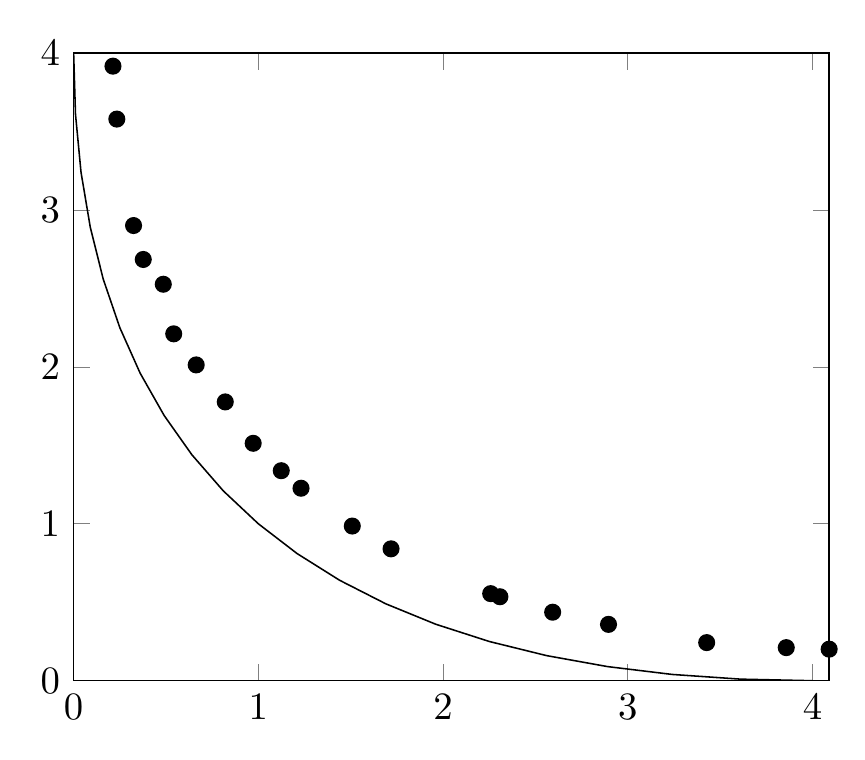
\begin{tikzpicture}[scale=1.4]
        \begin{axis}[enlargelimits=false]
            \addplot [] coordinates {
                (0.000000,4.000000) (0.010000,3.610000) (0.040000,3.240000) (0.090000,2.890000) (0.160000,2.560000) (0.250000,2.250000) (0.360000,1.960000) (0.490000,1.690000) (0.640000,1.440000) (0.810000,1.210000) (1.000000,1.000000) (1.210000,0.810000) (1.440000,0.640000) (1.690000,0.490000) (1.960000,0.360000) (2.250000,0.250000) (2.560000,0.160000) (2.890000,0.090000) (3.240000,0.040000) (3.610000,0.010000) (4.000000,0.000000) 
            };
            
            \addplot [only marks] coordinates {
                (4.089889,0.201051) (0.212879,3.916492) (1.718164,0.840462) (0.233704,3.579271) (2.257582,0.554891) (0.324342,2.900788) (0.541738,2.210647) (3.426797,0.242826) (2.895421,0.359023) (1.123887,1.338449) (2.593138,0.436579) (1.230869,1.226639) (0.971903,1.513040) (0.820711,1.776763) (2.307522,0.535176) (0.485212,2.526696) (3.857620,0.210809) (1.508379,0.985681) (0.376842,2.684529) (0.663446,2.012542) 
            };
        \end{axis}
    \end{tikzpicture}
\end{figure}